\section{Basic Methods}
\label{BasicM}
In order to get some basic understanding of the methods commonly used for iris classification the work presented in an article is implemented. The work implemented is the work of \cite{Khan2017a} described in \citep{Khan2017a}. In the work visible light images of the iris obtained by smartphones are processed and used to train different classifiers. The processing consists of a sequence of steps. The steps included are

\begin{itemize}
\item Iris Detection
\item Eyelid Suppression
\item Iris Normalisation
\item Noise Removal
\item Histogram Equalisation 
\item Feature Extraction
\item Training and Classification
\end{itemize}
\autoref{fig:ExWars} shows an example of an image from the database. Before the first step some simple preprocessing was done. The red channel is preserved and the other two other colour channels are neglected. This is done because this simulates the use of NIR light. The result is a greyscale image based on the red channel. In the following sections the implementation of each of the steps will be elaborated. 

\begin{figure}[h]
\centering
\begin{subfigure}{.47\textwidth}
\centering
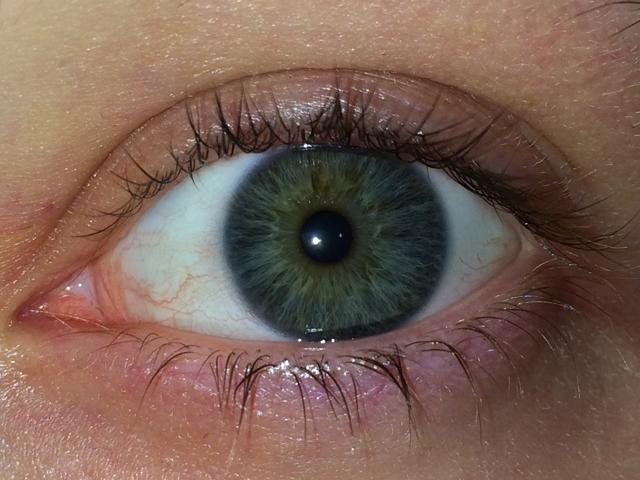
\includegraphics[width=0.90\textwidth]{IMG_1838.jpg}
\caption{Example of visible light image of an iris from the used database.}
\label{fig:ExWars}
\end{subfigure}
~
\begin{subfigure}{.47\textwidth}
\centering
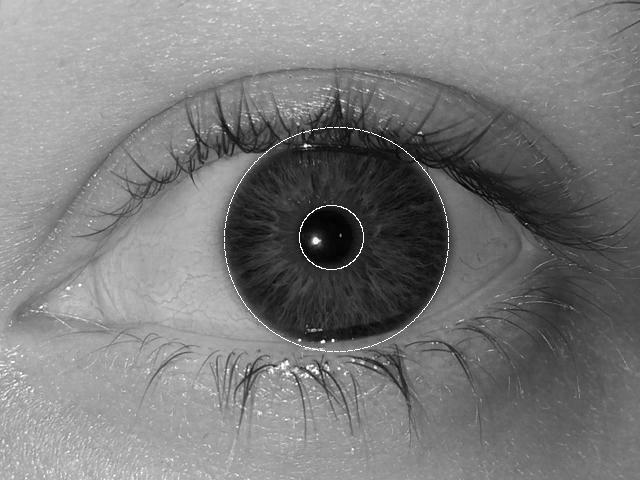
\includegraphics[width=0.90\textwidth]{0002left_13-marked.jpg}
\caption{The eye marked with the identified edges of the iris.}
\label{fig:MarkedI}
\end{subfigure}
\end{figure}



\subsection{Iris Detection}
The first step of processing is locating the iris. For this purpose Daugman's Integro-differential operator was used. The operator identifies the circular contour, which has the greatest change in intensity by varying the three parameters defining the circle. \autoref{fig:MarkedI} shows an example of the identified edges of the iris.



\subsection{Eyelid Suppression}

\subsection{Iris Normalisation}
For the normalisation Daugman's rubber sheet model is used. The purpose is to get a rectangular image of the iris, which corresponds to taking the annulus covered by the iris region, cutting it open and unfolding or stretching it to a rectangular shape. 

The model does this by mapping from polar coordinates based on radius and angle in the annulus to a rectangle where the angle is on the x-axis and the radius is on the y-axis of the image. 
This was implemented using a function in the library crated my Libor Masek.




\begin{figure}[h]
\centering
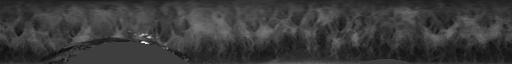
\includegraphics[width=\textwidth]{002polar.jpg}
\caption{The normalised image of the iris before applying functions.}
\label{fig:SimPolar}
\end{figure}

\subsection{Noise Removal}
Though the article uses several well known methods that are commonly used in processing of images of irises, there descriptions of the methods are quite inadequate. After obtaining the normalised iris the next step applied is noise removal. The purpose of the noise remover function is to remove noise occurring in the form of eyelashes covering parts of the iris. Usually the pixels showing the lashes will be among the darkest pixels. Since every image of the iris is different and how dark the iris is also varies, a threshold has to be identified adaptively. The article does not describe in depth how this is implemented, it simply states that some histogram analysis is done in order to obtain the lowest pixel values. \autoref{fig:histBif} shows the histogram of the normalised image before any noise removal. 
\begin{figure}[h]
\centering
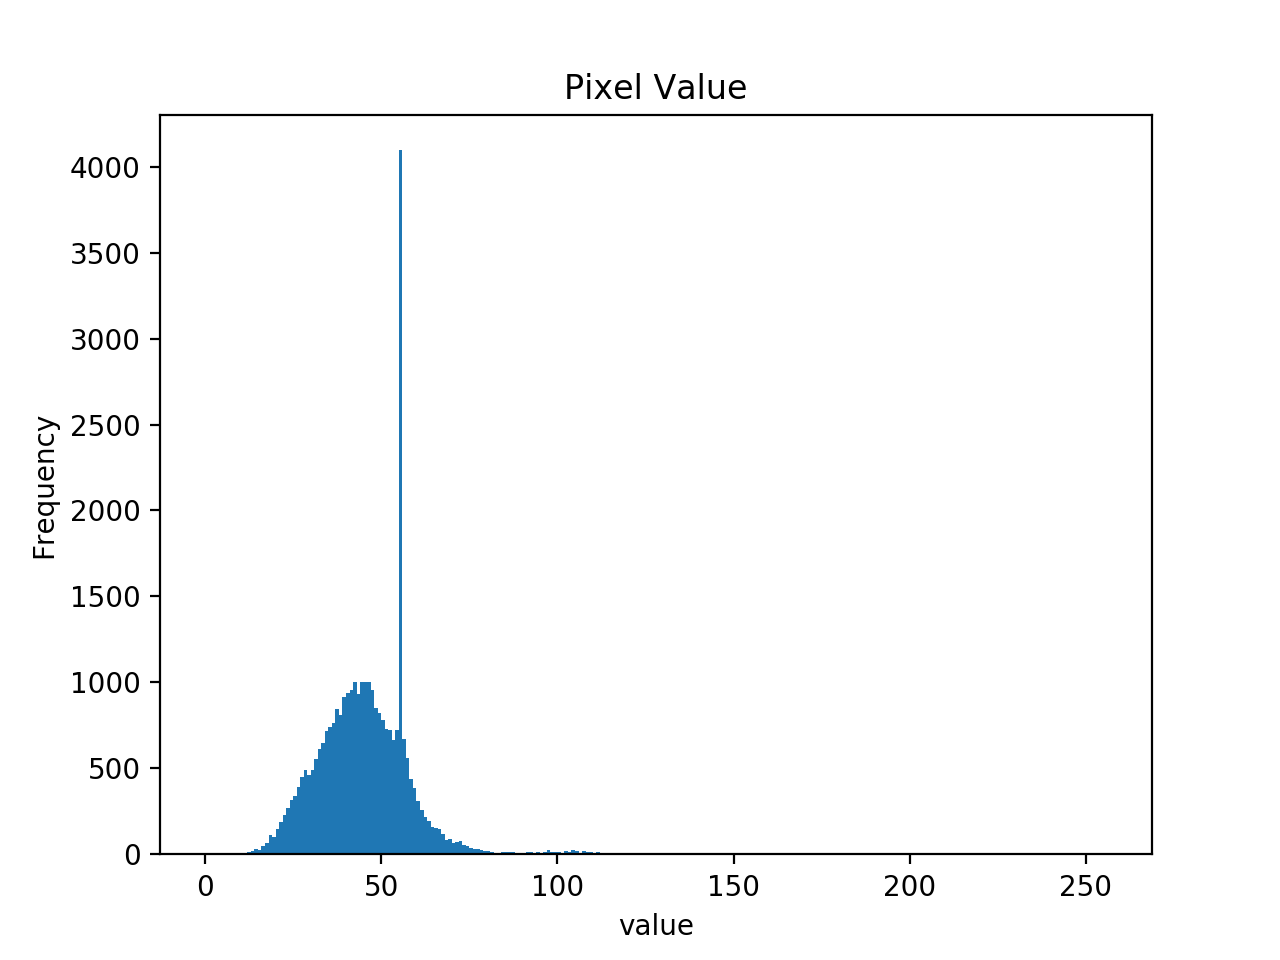
\includegraphics[width=0.7\textwidth]{hist_before.png}
\caption{The histogram before applying the functions.}
\label{fig:histBif}
\end{figure}
Because the information about the exact approach used in the article is inadequate, an adaptive algorithm was created. The algorithm implemented identifies a threshold value based on the histogram. This is done by first identifying the highest and lowest bin-value, which has a frequency of more than a specified "recognition value", which was set to 10 in this project. The recognition value is introduced to make sure outliers are not defining for the threshold. Afterwards the threshold is calculated by the formula in \autoref{eq:pix_threshold}, where "Fraction" is a parameter set manually defining how large a part of the identified pixel value range has to me thresholded. During the processing in this project "Fraction" was set to be equal $0.1$. 

\begin{equation}\label{eq:pix_threshold}
	\text{Threshold}=(\text({owVal})+\text{Fraction}\cdot\text{higVal-lowVal}
\end{equation}

After the threshold has been found it is applied to all pixels in the image. The pixels lower than the threshold are eliminated and have to be reconstructed from neighbouring pixels. Also here the article provides very limited information about the algorithm applied. Therefore an algorithm was implemented, which restores pixels from non-occluded neighbour regions. A part of the algorithm identifies the pixels with values lower than the threshold and saves the pixel coordinates of the pixels. The saved pixels are  reconstructed iteratively from neighbouring pixels following the 4-connectivity principle. The pixels are reconstructed when there are at least 2 neighbour pixels they can be reconstructed from. They are only reconstructed from pixels above the threshold, this can be pixels that initially were above the threshold, or it can be pixels that have already been reconstructed. The pixels are reconstructed by assigning the average of the neighbours with values above the threshold as the new pixel value. Once all thresholded pixels have been reconstructed the reconstructed image is returned.

Because the eliminated pixels are reconstructed only from pixels with a value higher than the threshold there are certain traits that can be expected in the histogram of the reconstructed image. One of the traits is that there is a flatline from 0 to the threshold value. A second trait is that a peak close to the threshold is likely to occur because the eliminated values are reconstructed from neighbours which are likely to be close to the value of the eliminated pixels. However, the plotted histogram after reconstruction is as shown in \autoref{fig:histSpill}.
\begin{figure}[h]
\centering
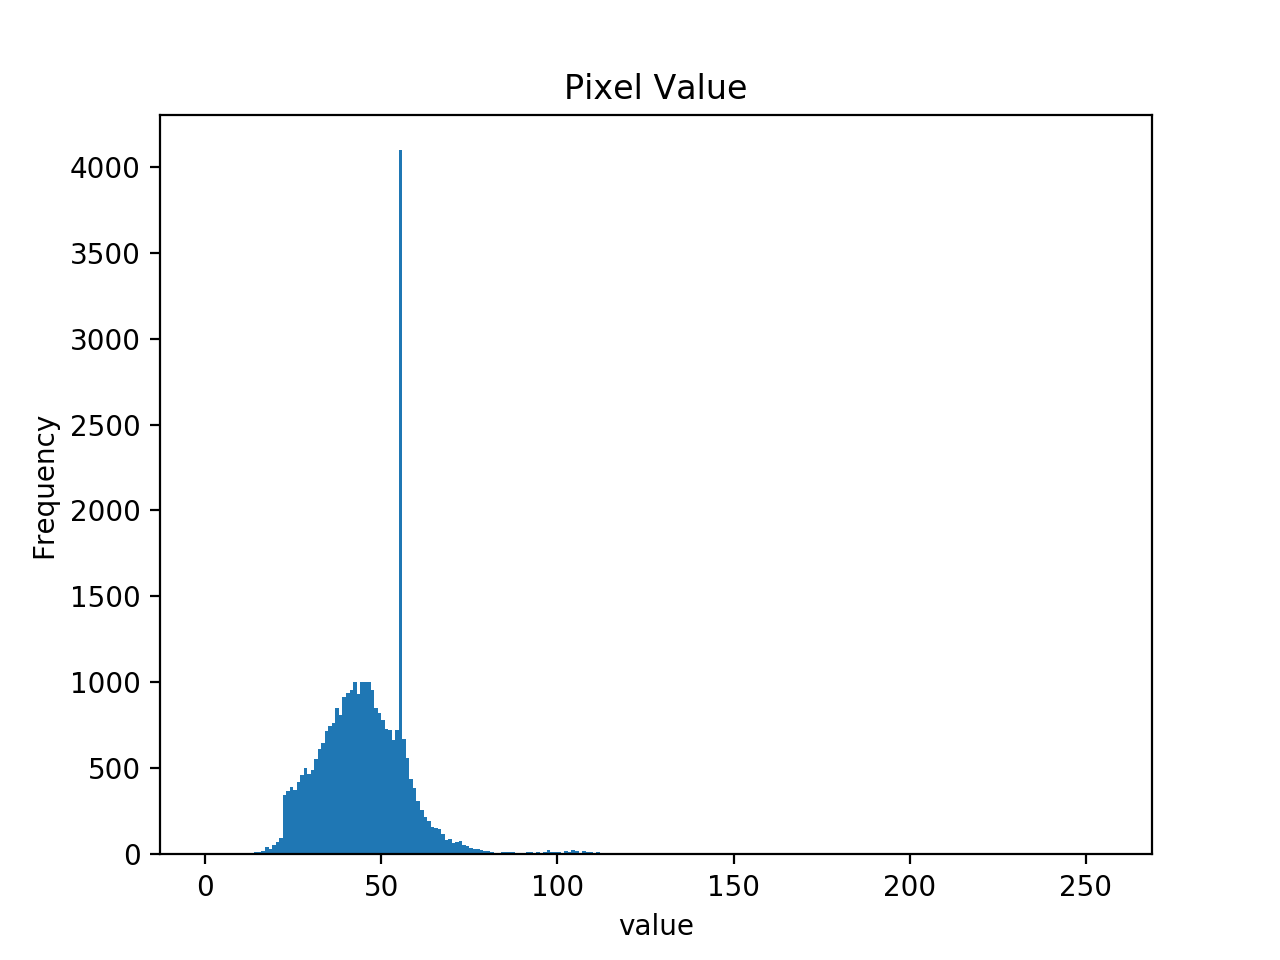
\includegraphics[width=0.7\textwidth]{hist_spill.png}
\caption{The histogram of the image after reconstruction of pixels.}
\label{fig:histSpill}
\end{figure}
As can be seen there is a peak as expected, however, there seem to be a "spill over" across the threshold to the lower values. By closer examination of the code it was discovered that this was caused due to a programming mistake. The mistake was that the values used for reconstruction were obtained from the original image and not from the reconstructed image. Once this mistake was corrected the histogram was as expected as shown in \autoref{fig:histFine}. 
\begin{figure}[h]
\centering
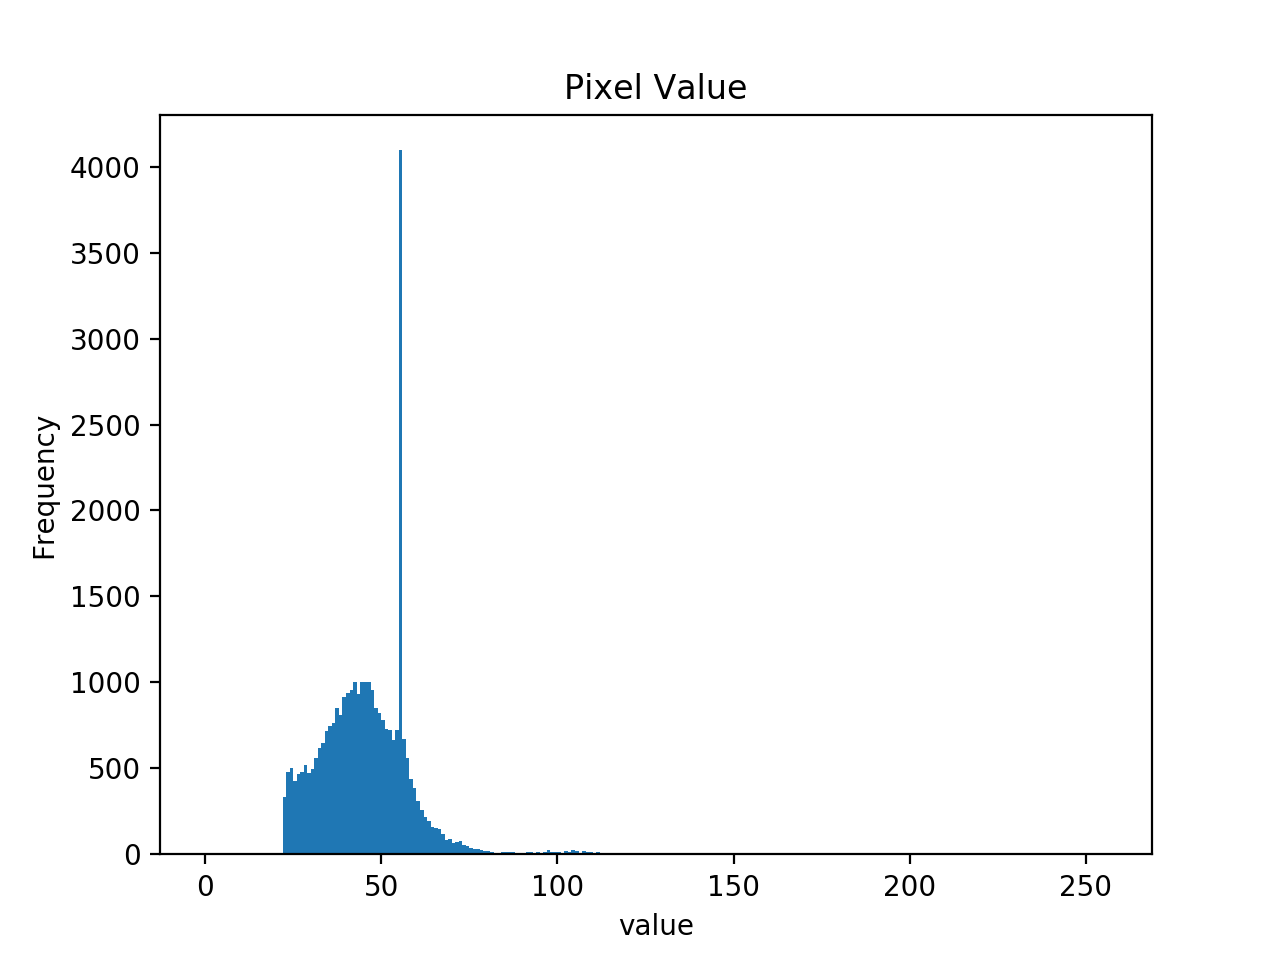
\includegraphics[width=0.7\textwidth]{hist_nicespacing.png}
\caption{The histogram of the image after applying the noise corrected remover function.}
\label{fig:histFine}
\end{figure}
In relation to the reconstruction of pixels it should be noted that it could have been done with 8-connectivity, and the iterative process could be split up so more steps, such that pixels are always constructed from as many neighbours as possible. This may give a better reconstruction, however, this has not been investigated. 
\subsection{Histogram Equalisation}
The histogram Equalisation

\begin{equation}\label{eq:hist_stretch}
	\text{New~pixelValue} (\text{pixelValue-lowVal})\cdot\frac{255}{\text{higVal-lowVal}}
\end{equation}


\begin{figure}[h]
\centering
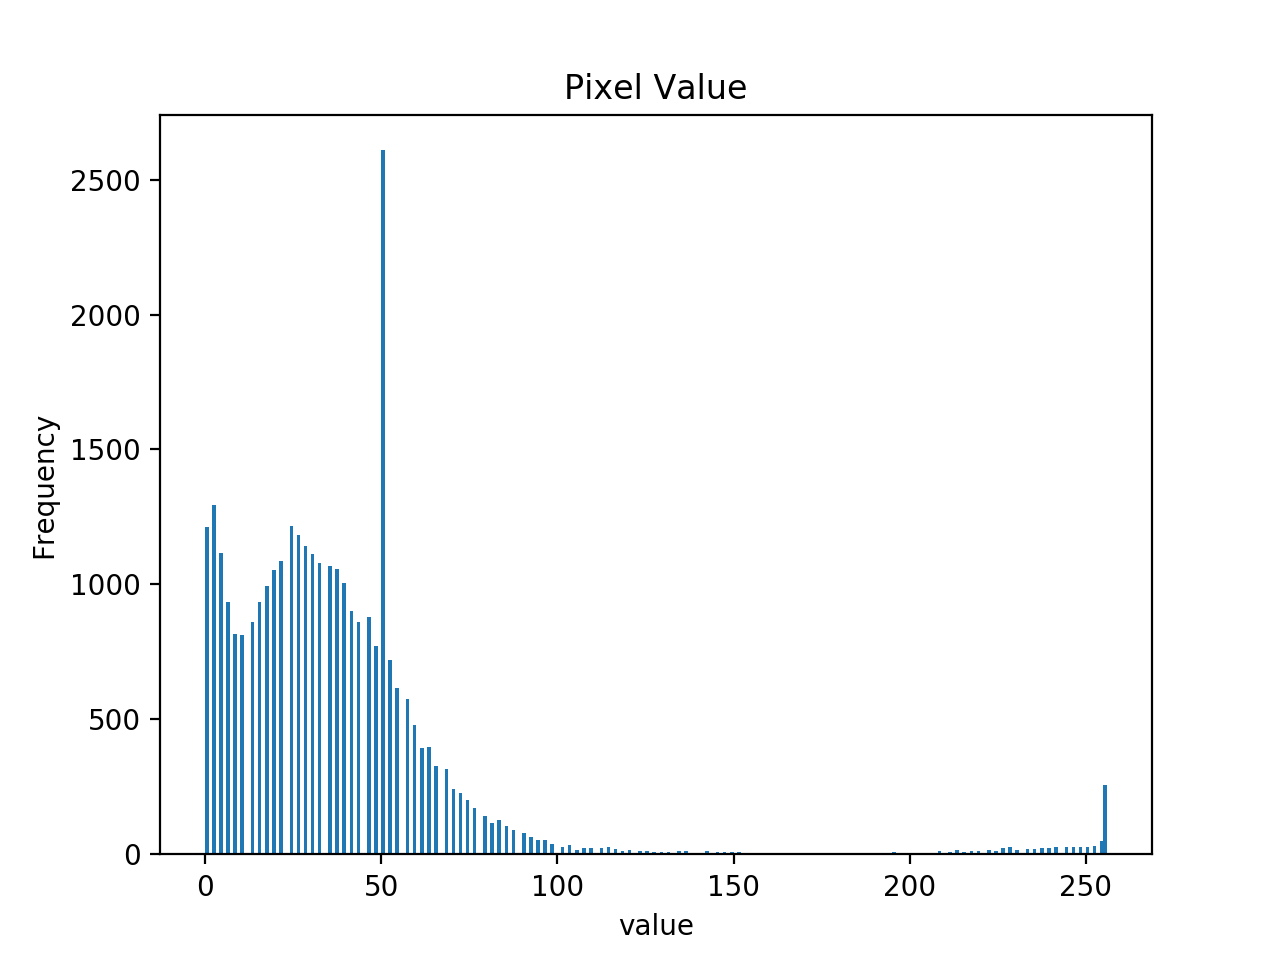
\includegraphics[width=0.7\textwidth]{hist_equal.png}
\caption{The histogram of the image after applying the equalise histogram function.}
\label{fig:histEq}
\end{figure}

\subsection{Feature extraction}


\subsection{Training and Classification}
For classification different classifiers were tested. 




Cross validation




